%%%%%%%%%%%%%%%%%%%%%%%%%%%%%%%%%%%%%%%%%%%%%%%%%%%%%%%%%%%%%%%%%%%%%
%
%  This is a sample LaTeX input file for your contribution to
%  the M&C2023 topical meeting.
%
%  Please use it as a template for your full paper
%    Accompanying/related file(s) include:
%       1. Document class/format file: mc2023.cls
%       2. Sample PDF/Postscript Figure: figure.pdf,figure.ps
%       3. A PDF file showing the desired appearance: mc2023_template.pdf
%       4. cites.sty and citesort.sty that might be needed by some users
%    Direct questions about these files to: buijsa@mcmaster.ca
%    Originals provided by brantley1@llnl.gov
%
%    Notes:
%      (1) You can use the "dvips" utility to convert .dvi
%          files to PostScript.  Then, use either Acrobat
%          Distiller or "ps2pdf" to convert to PDF format.
%      (2) Different versions of LaTeX have been observed to
%          shift the page down, causing improper margins.
%          If this occurs, adjust the "topmargin" value in the
%          mc2023.cls file to achieve the proper margins.
%
%%%%%%%%%%%%%%%%%%%%%%%%%%%%%%%%%%%%%%%%%%%%%%%%%%%%%%%%%%%%%%%%%%%%%


%%%%%%%%%%%%%%%%%%%%%%%%%%%%%%%%%%%%%%%%%%%%%%%%%%%%%%%%%%%%%%%%%%%%%
\documentclass[letterpaper]{mc2023}
%
%  various packages that you may wish to activate for usage
\usepackage{tabls}
\usepackage{cites}
\usepackage{epsf}
\usepackage{appendix}
\usepackage{ragged2e}
\usepackage[top=1in, bottom=1in, left=1in, right=1in]{geometry}
\usepackage{enumitem}
\setlist[itemize]{leftmargin=*}
\usepackage{caption}
\captionsetup{width=1.0\textwidth,font={bf,normalsize},skip=0.3cm,within=none,justification=centering}

% ELIMINATING WHITESPACE
\setlength{\belowcaptionskip}{-15pt}
\setlength{\abovedisplayskip}{4pt}
\setlength{\belowdisplayskip}{4pt}

\usepackage[colorlinks = true, linkcolor = black, urlcolor  = black, citecolor = black]{hyperref}
\usepackage{float} % for [H] option in figures

% GLOSSARIES
\usepackage[acronym,nomain,nonumberlist,nogroupskip,nopostdot]{glossaries} % for glossary of acronyms
\setacronymstyle{long-short}
\loadglsentries{glossary}
\makeglossaries
\renewcommand*{\glstextformat}[1]{\textcolor{black}{#1}} % make glossary color black

% This file contains custom commands that Lewis uses frequently in LaTeX documents

\usepackage{subcaption}
\usepackage{hyperref}
\hypersetup{colorlinks,allcolors=black}
% for more https://tex.stackexchange.com/questions/88400/hyperref-changing-the-linkcolor-locally-in-the-toc
\usepackage{amssymb}
\usepackage{bbm}

% matlab stuff
\usepackage{graphicx}
\usepackage{color}
\usepackage{matlab-prettifier}

%vector arrow
\usepackage{graphicx}
\newcommand{\cev}[1]{\reflectbox{\ensuremath{\vec{\reflectbox{\ensuremath{#1}}}}}}
% table packages
\usepackage{booktabs}
\usepackage{adjustbox}

% custom equation commands
\newcommand{\QOR}{\qquad \text{OR} \qquad}
\newcommand{\QAND}{\qquad \text{AND} \qquad}
\newcommand{\QTHUS}{\qquad \text{THUS} \qquad}
\newcommand{\QWITH}{\qquad \text{WITH} \qquad}
\newcommand{\QFOR}{\qquad \text{FOR} \qquad}
\newcommand{\QSO}{\qquad \text{SO} \qquad}
\newcommand{\QWHERE}{\qquad \text{WHERE} \qquad}
\newcommand{\QWHEN}{\qquad \text{WHEN} \qquad}
\newcommand{\LINE}{\par\noindent\rule{\textwidth}{0.4pt}\par}
\newcommand{\toinf}{\rightarrow\infty}
\newcommand{\tozero}{\rightarrow0}
\newcommand{\qeq}{\overset{?}{=}}
\newcommand{\ceq}{\overset{\checkmark}{=}}
\newcommand{\Poi}{\text{Poisson}}
\newcommand{\keff}{$k_{e\!f\!f}$}
\renewcommand{\epsilon}{\varepsilon} % squiggly epsilon

\def\brac#1{\{#1\}}
\def\Brac#1{\big\{#1\big\}}
\def\BRAC#1{\bigg\{#1\bigg\}}
\def\angbrac#1{\langle#1\rangle}
\def\Angbrac#1{\big\langle#1\big\rangle}
\def\ANGBRAC#1{\bigg\langle#1\bigg\rangle}
\usepackage{float}
% SI Units
\usepackage{siunitx}
\DeclareSIUnit\n{n}
\DeclareSIUnit\sp{sp}

\def\doubleunderline#1{\underline{\underline{#1}}}

\title{Verification of the Cardinal Multiphysics Solver for 1-D Coupled\\
Heat Transfer and Neutron Transport}

\raggedbottom % allows space at bottom of page, as opposed to verical justification
\author{%
  % FIRST AUTHORS
  %
  \textbf{L.I.~Gross$^1$, A.J.~Novak$^2$, P.~Shriwise$^2$, and P.P.H.~Wilson$^1$}\\
  $^1$University of Wisconsin -- Madison  \\
  1500 Engineering Drive, Madison, WI 53706 \vspace{6pt}\\
  $^2$Argonne National Laboratory \\
  9700 S Cass Avenue, Lemont, IL 60439\vspace{6pt} \\
  \url{ligross@wisc.edu}, \url{anovak@anl.gov}, \url{pshriwise@anl.gov}, \url{paul.wilson@wisc.edu}
}
%
% Insert authors' names and short version of title in lines below
%
\newcommand{\authorHead}{Gross et al.}
\newcommand{\shortTitle}{Verification of the Cardinal Multiphysics Solver}
%
%%%%%%%%%%%%%%%%%%%%%%%%%%%%%%%%%%%%%%%%%%%%%%%%%%%%%%%%%%%%%%%%%%%%%
%
%   BEGIN DOCUMENT
%
%%%%%%%%%%%%%%%%%%%%%%%%%%%%%%%%%%%%%%%%%%%%%%%%%%%%%%%%%%%%%%%%%%%%%
\begin{document}
\maketitle
\justify
\parskip 6pt plus 1 pt minus 1 pt

\begin{abstract}
Cardinal is a multiphysics software tool that couples OpenMC Monte Carlo transport and NekRS \gls{cfd} to the \gls{moose}. This
work verifies Cardinal for coupled neutron transport and heat conduction using a 1-D analytical solution from previous work by the
Naval Nuclear Laboratory. This numerical benchmark includes $S_2$ transport, Doppler-broadened cross sections, thermal conduction
and expansion, and convective boundary conditions. The goal of this work is to verify Cardinal's basic multiphysics modeling
capabilities for coupled neutronics and heat conduction. The benchmark provides analytical solutions for the temperature and flux
distributions, as well as the $k$-eigenvalue. Using these solutions, an $L_{2}$ error norm was computed for each spatial discretization:
namely finite element heat conduction mesh and Monte Carlo cells. The temperature error showed linear convergence on a log-log plot of
error vs. mesh element number, with a slope of $-0.9986$ ($R^2\approx 1.0$). Nearly all spatial flux predictions, except a few points
in the $N=250$ case, space were within $2\sigma$ of the analytical solution, for Monte Carlo cell counts between 50 and 1000. The
eigenvalue \keff~also agrees well with the benchmark value for each mesh size. The outcome of this work is verification of coupled
Monte Carlo-thermal conduction modeling using Cardinal.
\end{abstract}
\vspace{6pt}
\keywords{Cardinal, MOOSE, OpenMC, multiphysics, verification}

\section{INTRODUCTION}
\label{sec:intro}
With recent advancements in methods, software, and computing, high-fidelity, multiphysics \gls{ms} is becoming an important
component of the nuclear engineer's ``toolbox.'' These high-fidelity models substitute more conservative safety factors
with physics-based simulation. This can reduce uncertainty in analyses, enabling tighter margins to realize improved economics
and licensing certainty. However, analytical benchmarks and comparison to experimental data are required to assess the stability,
convergence, and accuracy of these high-fidelity models for reactor design and analysis.

Cardinal\footnote{\url{https://cardinal.cels.anl.gov/}} is an open-source code \cite{novak2022-cardinal}
that wraps OpenMC \cite{openmc} Monte Carlo particle transport and NekRS \cite{nekrs} \gls{cfd} within the \gls{moose}
\cite{lindsay2022moose} framework. This coupling brings high-fidelity multiphysics feedback to the \gls{moose} ``ecosystem.''
Cardinal couples OpenMC and NekRS to \gls{moose} simulations by copying data between the internal code data structures
(e.g. a vector of tally results in OpenMC) and a \texttt{MooseMesh}, or the unstructured mesh class in \gls{moose}. \gls{moose}'s
mesh-to-mesh interpolation system then communicates between the \texttt{MooseMesh} ``mirror'' of the external code's solution
and an arbitrary coupled \gls{moose} application in the form of boundary conditions (such as for conjugate heat transfer with
NekRS) or source terms (such as for volumetric heating with OpenMC). Convergence is obtained with Picard iteration.

For coupled neutronics-thermal-fluid simulations with OpenMC, each Picard iteration consists of several steps: 1)~a \gls{moose}
application (e.g. BISON, Pronghorn, NekRS via Cardinal, ...) solves for temperatures and densities; 2)~Cardinal transfers
temperatures and densities to the OpenMC model; 3)~OpenMC solves for the nuclear heating; and 4)~Cardinal transfers the tally
values back to the \texttt{MooseMesh} ``mirror.'' These steps continue until convergence criteria are achieved. In this work, we
pursue verification of these multiphysics aspects of Cardinal using a 1-D analytical benchmark from the Naval Nuclear Laboratory
\cite{analytical-benchmark}. This work does not require \gls{cfd}, and thus NekRS will be left out of the discussion from this
point on. However, we note that a companion paper in this conference does use NekRS's heat conduction solver for verification on
a different, fixed-source benchmark \cite{aya2023}.

The remainder of this paper is organized as follows. In Section \ref{sec:benchmark}, we summarize the analytical benchmark
modeled in this work. Section \ref{sec:model} then describes the Cardinal computational model of the benchmark. Section
\ref{sec:results} presents comparisons between Cardinal and the analytical benchmark. Finally, Section \ref{sec:conclusions}
presents conclusions and outlines ongoing and future efforts in the verification and validation of Cardinal.

\section{BENCHMARK PROBLEM DESCRIPTION}
\label{sec:benchmark}
The analytical benchmark couples three physics: $S_2$ neutron transport with Doppler broadening, heat conduction, and thermal
expansion. $S_{2}$ transport restricts the neutron direction to only the $\pm x$ direction. A summary of the governing \glspl{ode}
and boundary conditions in the 1-D slab is shown in Figure \ref{fig:slab_diagram}. The assumed model for thermal conductivity has
already been inserted into the energy conservation equation.
\begin{figure}[H]
    \centering
    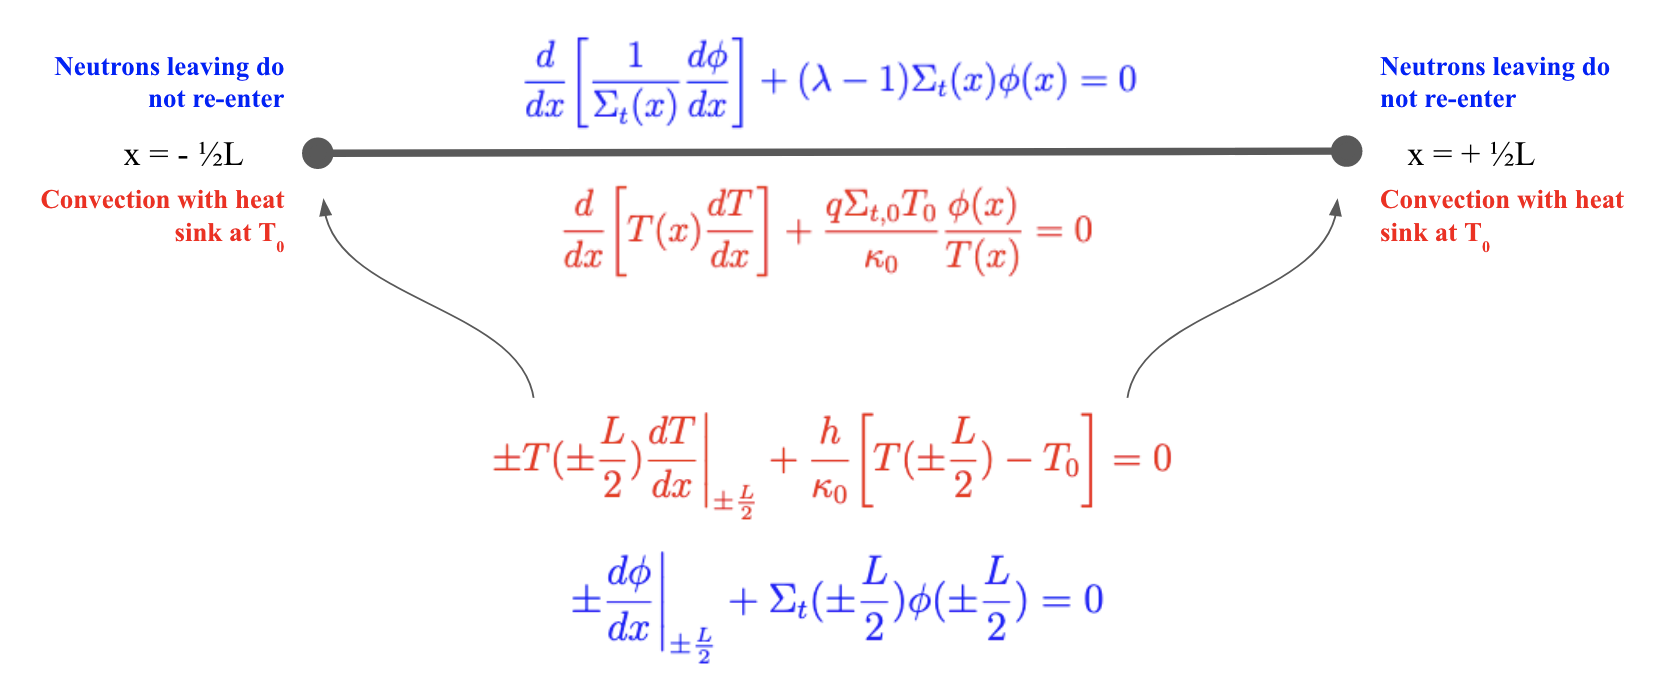
\includegraphics[width=0.85\linewidth]{figures/1D_Benchmark_Diagram.png}
    \caption{The domain, \glspl{ode}, and boundary conditions for the slab.}
    \label{fig:slab_diagram}
\end{figure}

This benchmark uses a one-group assumption for the neutron cross sections. As neutrons transport, heat from fission events deposits
volumetric power in the slab, causing thermal expansion and affecting the temperature distribution; thermal expansion is restricted
to only the $x$-direction. This slab elongation feeds back into neutronics and heat conduction by influencing the domain length and
material density. The slab has convective boundary conditions at the endpoints $x=\pm \frac{L}{2}$ with the heat sink temperature
$T_{0}$. The Doppler-broadened, total, microscopic cross section follows an inverse-root temperature relationship,
\begin{equation}
    \sigma_{t}(x) = \sigma_{t,0}\sqrt{\frac{T_{0}}{T(x)}}.
\end{equation}
Due to thermal expansion, the slab density varies as
\begin{equation} \label{sec:intro:density}
    \rho(x) =  \rho_{0} \sqrt{\frac{T_{0}}{T(x)}}.
\end{equation}
This gives a Doppler-broadened, macroscopic, total cross section that accounts for changes in density due to temperature as
\begin{equation}\begin{aligned} \label{sec:intro:doppler}
    \Sigma_{t}(x) =&\  \frac{\rho_{0}\sigma_{t,0} N_{A}}{A} \frac{T_{0}}{T(x)}\\
    =&\  \Sigma_{t,0}\frac{T_{0}}{T(x)} ,
\end{aligned}\end{equation}
where $ \sigma_{t,0}$ is the total microscopic cross section at $T_{0}$, $N_{A}$ is Avogadro's number, and $A$ is the mass number
of the medium. The conduction equation governs energy conservation in the slab and can be described in terms of the thermal conductivity
$\kappa$, the energy released per reaction $q$, the total macroscopic cross section $\Sigma_{t}$, and the neutron flux $\phi$,
\begin{equation}
     \frac{d}{dx}\left\lbrack\kappa(T)\frac{dT(x)}{dx}\right\rbrack + q \Sigma_{t}(x)\phi(x) = 0.
\end{equation}
Note that typically $q$ represents the energy per fission, but in this benchmark, $q$ is per total reaction.

By defining the problem in this way, the differential equations for thermal conduction and neutron transport have similar forms,
suggesting that it may be possible that the temperature and flux are related by a constant, $T(x)=f\phi(x)$. This
assumption is satisfied by manipulating the \glspl{ode}, inserting the cross section temperature dependence, and matching
coefficients so that the two \glspl{ode} are of the same form. The matching of coefficients imposes two constraints that give
equations for the total, microscopic cross section $\sigma_{t,0}$ and the heat transfer coefficient $h$, in terms of the slab
parameters. An important consequence of this problem is that the fission power is uniform throughout the geometry (but the
flux is not). For full details on the analytical solution's derivation, see \cite{analytical-benchmark}.

\section{COMPUTATIONAL MODEL}\label{sec:model}
This section describes the OpenMC and \gls{moose} computational models, followed by the coupling's convergence criteria and
a description of the mapping between OpenMC and \gls{moose} geometries. When the benchmark model was completed, Cardinal did
not yet support moving geometries in OpenMC. Instead of modeling thermal expansion using thermomechanics, our simulation uses
the analytical solution for the equilibrium length $L$ from \cite{analytical-benchmark} that accounts for all three physics
effects. This simulation accounts for changes in density due to temperature by using the total, macroscopic cross section\ --\
which absorbs density to become a $\frac{1}{T}$ dependence\ --\ as was mentioned in Section \ref{sec:benchmark}. We note, in
a companion paper in this conference \cite{novak-2023}, that Cardinal now supports mesh-based geometry (and deforming-mesh
problems) through the DAGMC plugin, and hence incorporating the thermomechanics feedback will be included in our future work.

\subsection{OpenMC Model}
\label{sec:model:OpenMC}
The slab is divided evenly into $N$ identically-shaped, rectangular cells along the $x$-dimension; the cases here are $N=[5, 10,
25, 50, 100, 250, 500, 1000]$ cells.  The geometry used in OpenMC must be three-dimensional, despite the benchmark being a 
one-dimensional problem. In general, reflective boundary conditions can be used to remove dimensions from a problem. Thus, this
benchmark can be represented with vacuum boundary conditions at $x=\pm \frac{L}{2}$ and reflective boundary conditions at the $y$
and $z$ boundaries.  To simplify normalization of the power integral in Equation (19) of the benchmark, the geometry has $1$ cm
dimensions in the $y$ and $z$ directions \cite{analytical-benchmark}. Figure \ref{fig:slab_diagram} shows a diagram of the 1-D
geometry, governing equations, and boundary conditions for the different physics.

The benchmark's one-group assumption was satisfied using OpenMC's multigroup mode. Since the benchmark uses a fictitious material
with a known function for the temperature dependence, the simulation took advantage of OpenMC's capability for user-defined
cross sections via the \texttt{XSdata} class. The cross section for each reaction was specified for 50 evenly spaced temperatures
between 308 K and 358 K (a range slightly larger than, but including the  analytical temperature range from the benchmark) and was
exported to a library. Then, when running OpenMC in multigroup mode, that library is loaded to determine the appropriate cross
section in each region as temperature changes from iteration to iteration. For a temperature $T$ between two library data points,
we use the nearest temperature available.

OpenMC required slight source code modifications to accommodate $S_2$-like transport. While reflective boundary conditions in the
$y$ and $z$ directions are necessary, in general, to establish a 1-D problem, in this benchmark particles only move in the $\pm x$
direction. In typical OpenMC simulations, the physics of each reaction describes the scattering dynamics. The Monte Carlo algorithm
is agnostic to the direction particles move, but it is not typically constrained to a discrete directional distribution. However,
when modeling this benchmark, any history with a particle moving perpendicular to the $x$-direction would attenuate particles in less
$x$-distance than if particles were constrained to either $\pm x$. To address this, we first use OpenMC's \texttt{PolarAzimuthal}
distribution to restrict the birth direction of particles to the $\pm x$ direction. We then also modified OpenMC in a patched branch
to mimic $S_{2}$ transport in two ways. First, when determining the angular cosine of scattering events, $\mu$, particles either
continue forward ($\mu=1$) or are back-scattered ($\mu=-1$) with equal probability, as opposed to sampling the reaction physics
for $\mu$. Second, since the simulation uses $k$-eigenvalue mode, neutrons born in subsequent generations of the simulation also
need to have their angular birth distributions restricted to $\pm x$.

As with any Monte Carlo eigenvalue method, each Picard iteration requires sufficient inactive batches to converge the fission source,
followed by sufficient active batches to accumulate the relevant tally results. A Shannon Entropy \cite{brown-entropy-2006} study for
this system was conducted on the 1000 cell case and found that the Shannon Entropy converges after about 5 inactive batches. While this
may seem like a low number, the problem is 1-D and the initial guess provided to OpenMC is a uniform distribution, which is the same
shape as the actual converged solution. The $k$-eigenvalue simulation used 50,000 particles per batch, with 50 inactive batches and
100 active batches for every case.

For simplicity, we always run 200 Picard iterations, though more advanced metrics in Cardinal can be used for programmatically
evaluating coupled physics convergence. Once the temperature was converged following 200 Picard iterations, a final OpenMC run was
performed using the temperature distribution produced from the last Picard iteration with 250,000 particles per batch and the same
number of batches.

Cardinal kept track of a few tallies in order to compare to the analytical solution: a flux cell tally, a fission heating (kappa-fission)
cell and global tally, and the eigenvalue \keff. Though flux and the eigenvalue are the only neutronics quantities to compare with the
benchmark, these other tallies are needed in order to compute a source strength. For an eigenvalue problem, the tally normalization relies
on a source strength, $S$, related to the total system power:
\begin{equation} \label{eq:source_strength}
   S = \frac{P}{H} \left[\frac{\textrm{sp}}{\textrm{s}} \right]
\end{equation}
where $P=10^{22} \frac{\textrm{eV}}{\textrm{s}}$ is the slab integrated power from the benchmark and $H \left[\frac{\textrm{eV}}{\textrm{sp}} \right]$
is the total tallied fission heating tally, where ``sp'' indicates ``source particle.'' Each tally must be multiplied by this source strength to
convert to physically meaningful units. Since OpenMC does not report volume-normalized tallies, it is necessary to divide by the cell volume
for quantities such as neutron flux and volumetric heating.

\subsection{MOOSE Heat Conduction Model}
\gls{moose} is used to solve for the temperature distribution within the slab via the Heat Conduction Module. In this \gls{moose}
model, a mesh is used that has identical dimensions to the cells used in the OpenMC model. While this is not required by Cardinal,
it allows for 1:1 feedback between the temperature computed in \gls{moose} and the heat source computed in OpenMC (and is
adequate for this geometrically simple benchmark). \gls{moose} solves the conduction equation using the \gls{fem}:
\begin{equation}\label{eq:conduction}
    - \nabla \cdot [\kappa_{s}(\mathbf{r},T_{s}) \nabla T_{s}(\mathbf{r})] = \dot{q}_{s},
\end{equation}
where $\kappa_{s}$ is the thermal conductivity in the solid and $\dot{q}_{s}$ is the heat source, in this case from fission. The
boundary conditions used by \gls{moose} match the temperature boundary conditions in red shown in Figure \ref{fig:slab_diagram}.
\gls{moose} is coupled to OpenMC by receiving the heat source in each element from the fission heating tally. During each iteration,
\gls{moose} recomputes the temperature distribution from the heat source and boundary conditions, and then sends the temperatures
back to OpenMC for the next transport solve.

\subsection{Convergence Criteria}
The \gls{moose} heat conduction solve used a \gls{jfnk} iterative method, with $10^{-7}$ for absolute tolerance and $10^{-9}$ for
relative tolerance. The Monte Carlo method is a stochastic method, so convergence is achieved by using an appropriate number of
batches and histories per batch. The configurations used here were discussed in Section \ref{sec:model:OpenMC}.

In terms of converging global iterations across all single physics, each case used 200 Picard iterations. To assist with
convergence of Monte Carlo quantities, Robbins-Monro relaxation was applied to the flux and fission heating tallies. This updates the
quantities of interest for the $n+1$th iteration as an average over the previous $n$ Monte Carlo solutions \cite{dufek}.
The relaxed flux at iteration $n$ is computed via
\begin{equation}\label{eq:Robbins-Monro}
    \Phi_{n} = \frac{1}{n+1} \sum_{i=0}^{n} \phi_{i},
\end{equation}
where $\Phi_{n}$ is the relaxed flux at step $n$ and $\phi_{i}$ is the flux output from the $i$th Monte Carlo solve. In order to assess
the convergence of each physics, we plotted error versus mesh element size and compared numerical versus analytical solutions in each
mesh element. These will be shown in Section \ref{sec:results}.

In this benchmark, a high number of Picard iterations was used in order to ensure convergence, but other modelers may not want to incur
the computational cost of running 200 Picard iterations. \gls{moose} provides steady-state detection as an alternate way of detecting
convergence. By setting a steady-state tolerance, \gls{moose} will iterate until the solution norm changes by less than this tolerance.
In Cardinal, OpenMC and NekRS variables are ``external" to other \gls{moose} non-linear variables. These auxiliary variables may include
some variables that should not be included in the steady-state detection (such as field variables storing the OpenMC cell ID, which does
not change with iteration but are sometimes used for diagnostics). This can trick the steady-state detection into ``detecting" convergence
faster than it should. Thus, this feature was not adopted for this work, though a new issue was opened in the MOOSE repository to allow
the user to control which auxiliary variables are used to assess convergence.  As long as the user removes any auxiliary variables not
used for coupling, they could rely on steady-state detection instead.

\subsection{Data Mapping}
Cardinal does not require the geometry models used in each single-physics sub-application to exactly match the meshes/geometry used in
other coupled codes. At the beginning of every Cardinal simulation, a mapping between \gls{moose}'s mesh and other geometry representations
is established. For a \gls{moose}-OpenMC coupling, the centroid of every MOOSE mesh element is mapped to a corresponding OpenMC cell using
OpenMC's find-cell routines. Cardinal then creates a tally for every user-requested type in each of the regions of OpenMC that a \gls{moose}
centroid falls in. This mapping is used for transferring relevant quantities back and forth between Picard iterations. 

For this simulation, the \gls{moose} geometry and OpenMC geometries were intentionally created to have the same dimensions so that the
mapping is 1:1. Each region in the \texttt{MooseMesh} computes a temperature and sends it to a geometrically identical OpenMC region.
This same region in an OpenMC solve computes a heat source via the fission heating tally and sends it back to \gls{moose} for the next
conduction solve. Again, we want to emphasize that this strict 1:1 mapping is {\it not} mandatory in Cardinal, and rather a general
centroid-based, non-conformal, many-to-one mapping from elements to cells can be used. In order to explore the convergence with spatial
resolution, eight different cases were analyzed with $N=[5, 10, 25, 50, 100, 250, 500, 1000]$ spatial elements/cells in both \gls{moose}
and OpenMC.

\section{RESULTS}\label{sec:results}
The results to compare with the benchmark are the temperature distribution, flux distribution, and $k$-eigenvalue. The benchmark provides
analytical solutions for all of these quantities. An example temperature and flux distribution is shown in Figure \ref{fig:temp_flux_50}
for the 50 mesh element case. In order to assess the accuracy of the numerical quantities and verify that refining the mesh increases the
accuracy, the analytical solution was used to compute an $L_{2}$ error norm for temperature and flux. The error, $\epsilon_{T}$, is given by
\begin{equation}
    \epsilon_{T} = \frac{|| T_{a} - T_{x} ||_{2}}{|| T_{a} ||_{2}},
\end{equation}
where $T_{a}$ is the analytical solution evaluated at the $x$-centroid of each mesh element, and $T_{x}$ is the temperature computed for that
voxel from the multiphysics simulation. The same convergence test was used on the flux solution as well. Using the same notation convention,
the flux error norm, $\epsilon_{\phi}$, is defined as
\begin{equation}
    \epsilon_{\phi} =  \frac{|| \phi_{a} - \phi_{x} ||_{2}}{|| \phi_{a} ||_{2}}.
\end{equation}
Figure \ref{fig:error_study} shows the temperature and flux error norms as a function of the number of mesh elements or cells.
\begin{figure}[H]
    \centering
    \begin{subfigure}[b]{0.395\linewidth}
        \centering
        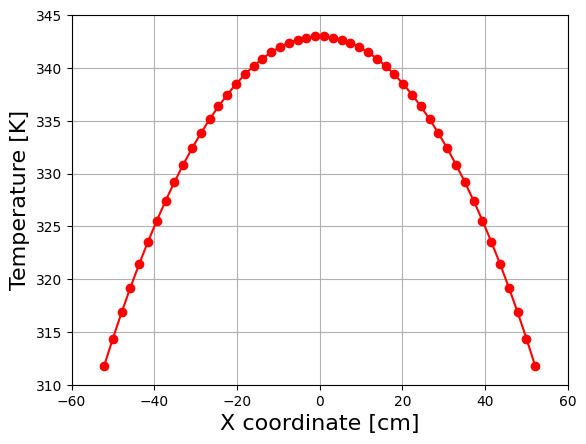
\includegraphics[height=0.7\linewidth]{figures/temp_50.png}
        \caption{Temperature profile for 50 elements.}
        \label{fig:temp_50}
    \end{subfigure}
    \begin{subfigure}[b]{0.395\linewidth}
    \centering
        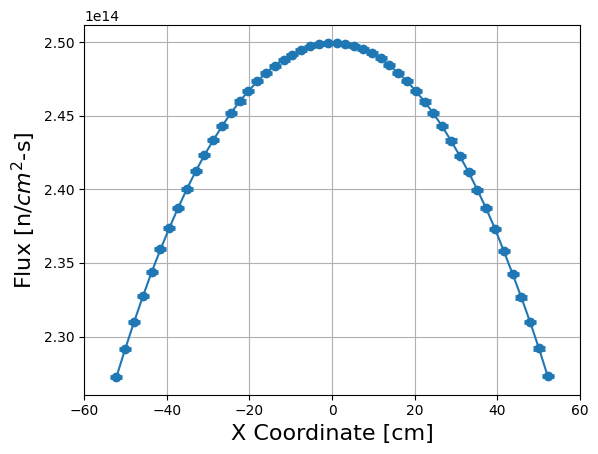
\includegraphics[height=0.7\linewidth]{figures/flux_50.png}
        \caption{Flux profile for 50 elements.}
        \label{fig:flux_50}
    \end{subfigure}
    \par\bigskip
    \caption{Numerical solutions for 50 mesh elements. The error bars show the relative error of the flux, which are
    nearly smaller than the circular marker sizes.}
    \label{fig:temp_flux_50}
\end{figure}
\begin{figure}[H]
    \centering
    \begin{subfigure}{0.395\linewidth}
        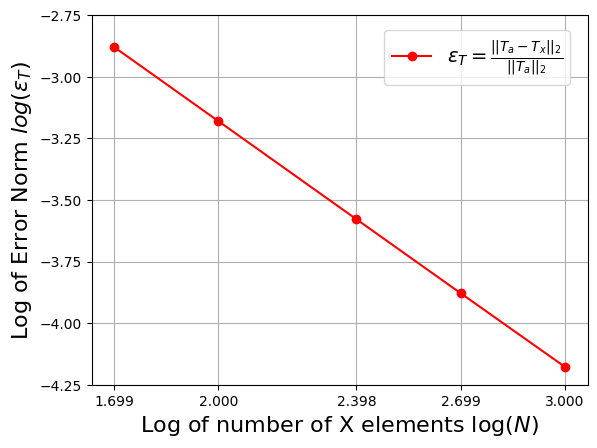
\includegraphics[width=\linewidth]{figures/temp_error_norms.png}
        \caption{Temperature error norms.}
        \label{fig:temp_err}
    \end{subfigure}
    \begin{subfigure}{0.395\linewidth}
        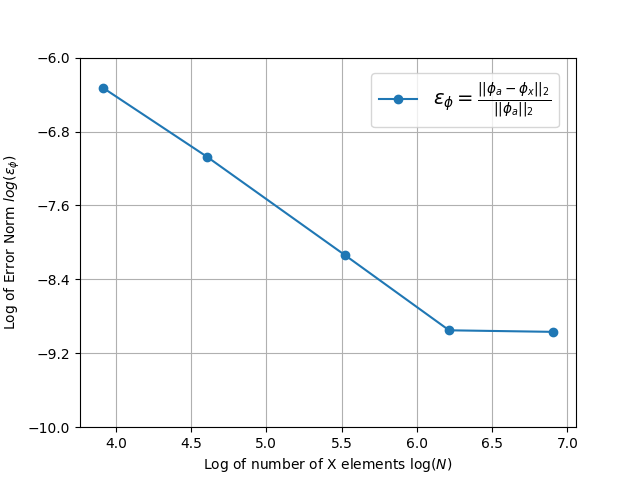
\includegraphics[width=\linewidth]{figures/flux_error_norms.png}
        \caption{Flux error norms.}
        \label{fig:flux_err}
    \end{subfigure}
    \par\bigskip
    \caption{Error norms as a function of heat conduction mesh element count and OpenMC cell count, respectively.}
    \label{fig:error_study}
\end{figure}
For the temperature distributions, linear convergence is achieved, as the slope of the temperature line in Figure \ref{fig:error_study} is
$-0.9986$ ($R^2\approx1.0$). The flux error does not appear to follow a linear pattern for the whole domain like the temperature error does.
The first four points decrease as the number of cells used increases, but after that the errors do not continue to behave linearly. The slope
of the first four points is $-1.381$ ($R^2=0.9814$). The flux error appears to stagnate after $50$ cells, suggesting that the error will not
improve considerably by increasing cell number because other error components dominate (e.g. stochastic noise, error from a cross section
library at 50 temperatures, etc.). At this point, the cases will be categorically referred in two groups: coarse ($5$, $10$, $25$) and fine
($50$, $100$, $250$, $500$, $1000$).

While the $L_2$ error norm of the flux does not exhibit convergence in the same way that the temperature does, the results do compare favorably
with the analytical results throughout the domain and for all spatial resolutions in the fine group. The ratio between the computed quantity,
$C$, and the expected answer, $E$, for the temperature in each element and flux in each cell are shown for all fine cases in Figure \ref{fig:fine_ce}.
A black line at $C/E = 1$ is marked in each plot indicating perfect agreement. Note the scales of the $y$-axes - the temperature is everywhere
being predicted to within 0.006\% (for the coarsest temperature mesh) and flux is everywhere being predicted to within 0.05\%.
\begin{figure}[H]
    \centering
    \begin{subfigure}{0.45\linewidth}
        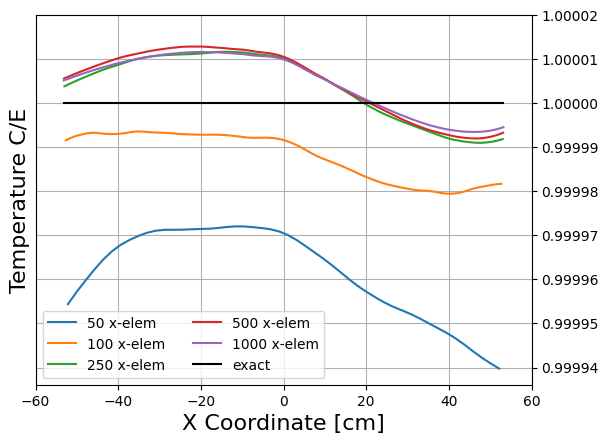
\includegraphics[width=\linewidth]{figures/fine_temp_num_to_analy_ratios.png}
        \caption{Fine temperature $C/E$.}
        \label{fig:fine_temp_ce}
    \end{subfigure}
    \begin{subfigure}{0.45\linewidth}
        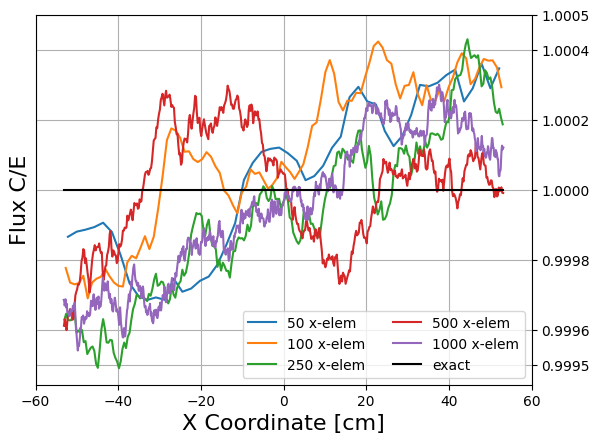
\includegraphics[width=\linewidth]{figures/fine_flux_num_to_analy_ratios.png}
        \caption{Fine flux $C/E$.}
        \label{fig:fine_flux_ce}
    \end{subfigure}
    \par\bigskip
    \caption{$C/E$ for fine cases.}
    \label{fig:fine_ce}
\end{figure}
As the mesh refinement increases, the $C/E$ results trend towards the ideal. For comparison, the coarser cases' $C/E$ results are
included in Figure \ref{fig:coarse_ce}. The coarse cases' errors are a few orders of magnitude larger than the fine cases. A significant
improvement in agreement can be seen between each coarse case.
\begin{figure}[H]
    \centering
    \begin{subfigure}{0.45\linewidth}
        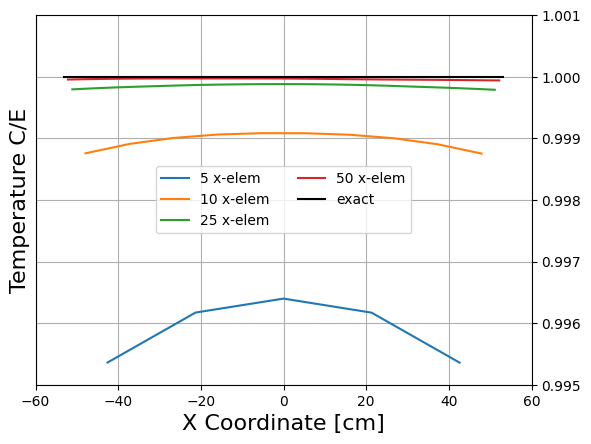
\includegraphics[width=\linewidth]{figures/coarse_temp_num_to_analy_ratios.png}
        \caption{Coarse temperature $C/E$.}
        \label{fig:coarse_temp_ce}
    \end{subfigure}
    \begin{subfigure}{0.45\linewidth}
        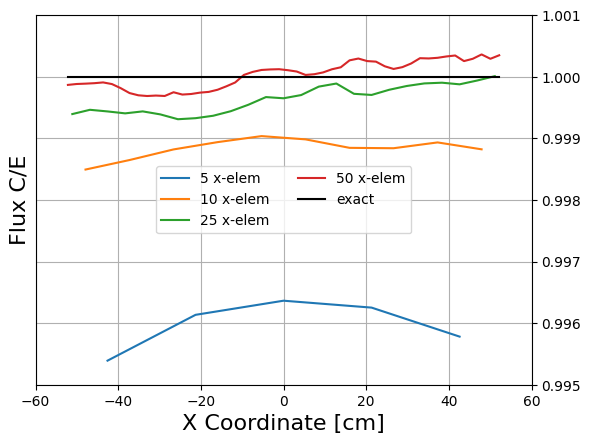
\includegraphics[width=\linewidth]{figures/coarse_flux_num_to_analy_ratios.png}
        \caption{Coarse flux $C/E$.}
        \label{fig:coarse_flux_ce}
    \end{subfigure}
    \par\bigskip
    \caption{$C/E$ for coarse cases.}
    \label{fig:coarse_ce}
\end{figure}
The temperature $C/E$ ratio is computed using \gls{fem}, but since the flux uses a stochastic approach, its $C/E$ depends on two quantities with
uncertainty. The flux from OpenMC $\hat{\phi}$ has uncertainty $\sigma_{\hat{\phi}}$ and the fission heating tally $\hat{H}$ has uncertainty
$\sigma_{\hat{H}}$. Writing the flux $C/E$ explicitly gives
\begin{equation}\begin{aligned}\label{eq:CE_formula}
    C/E =&\ 
    \frac{P\hat{\phi}}{V_{cell}\hat{H}\phi_{A}}\\ =&\  \frac{S\hat{\phi}}{V_{cell}\phi_{A}},
\end{aligned}\end{equation}
where $V_{cell}$ is the tallied region's volume and $\phi_{A}$ is the analytical flux. Propagating both errors:
\begin{equation}\label{eq:sigma_ce_def}
    \sigma_{C/E}^2 =
    \left( \frac{\partial C/E}{\partial\hat{\phi}} \right)^2 \sigma_{\hat{\phi}}^2  +
     \left( \frac{\partial C/E}{\partial \hat{H}} \right)^2 \sigma_{\hat{H}}^2 .
\end{equation}
Now denote $\phi$, $\sigma_{\phi}$, $H$, and $\sigma_{H}$ as the quantities with physical units, i.e. the OpenMC outputs multiplied by the source
strength and divided by volume. Evaluating the derivatives and simplifying gives
\begin{equation}\label{eq:sigma_CE_physical_units}
    \sigma_{C/E}^2 =
    \left(\frac{\sigma_{\phi} }{\phi_{A}} \right)^2 +
     \left( \frac{\phi}{\phi_{A}}\frac{V_{cell}}{P}\sigma_{H} \right)^2.
\end{equation}
Figure \ref{fig:ce_error_bars} shows individual $C/E$ with $2\sigma$ error bars (95\% confidence interval) for all the fine cases. Nearly all points
are within $2\sigma$, indicating that Cardinal is computing a correct flux distribution, within statistical uncertainty. Only a handful of points in
the $N=250$ case appear to be outside the error bars, but all other cases are fully contained. The coarse cases are excluded, as they are, expectedly,
outside the $2\sigma$ error bars.
\begin{figure}[H]
    \centering
    \begin{subfigure}{0.405\textwidth}
        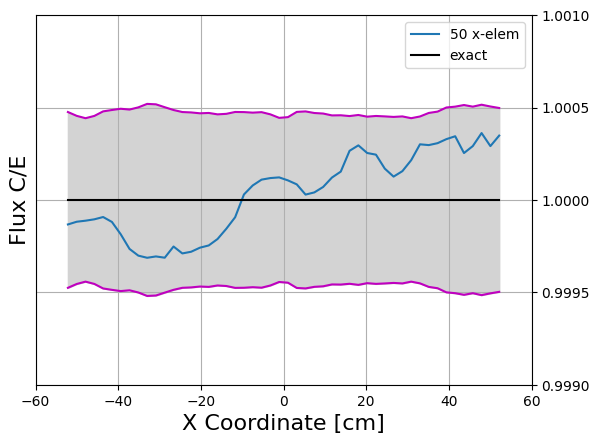
\includegraphics[width=\linewidth]{figures/50_flux_CE_error_bars.png}
        \caption{$N=50$}
        \label{fig:s1}
    \end{subfigure}
    \begin{subfigure}{0.405\textwidth}
        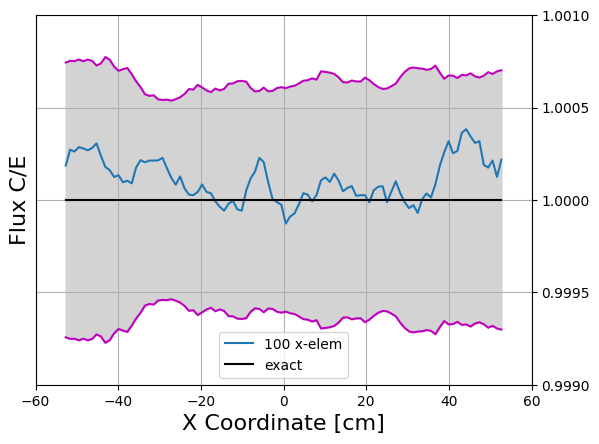
\includegraphics[width=\linewidth]{figures/100_flux_CE_error_bars.png}
        \caption{$N=100$}
        \label{fig:s2}
    \end{subfigure}
    \par\bigskip
    \begin{subfigure}{0.405\textwidth}
        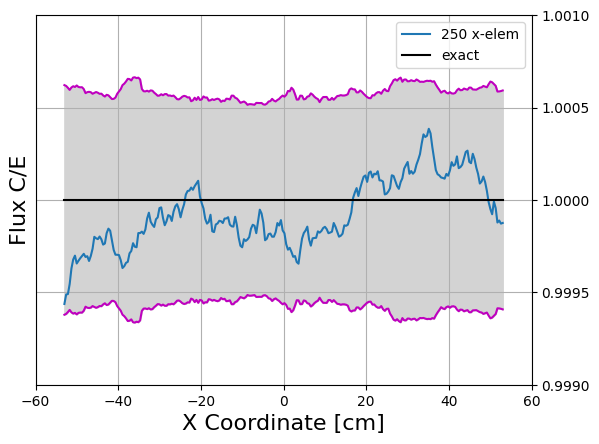
\includegraphics[width=\linewidth]{figures/250_flux_CE_error_bars}
        \caption{$N=250$}
        \label{fig:s3}
    \end{subfigure}
    \begin{subfigure}{0.405\textwidth}
        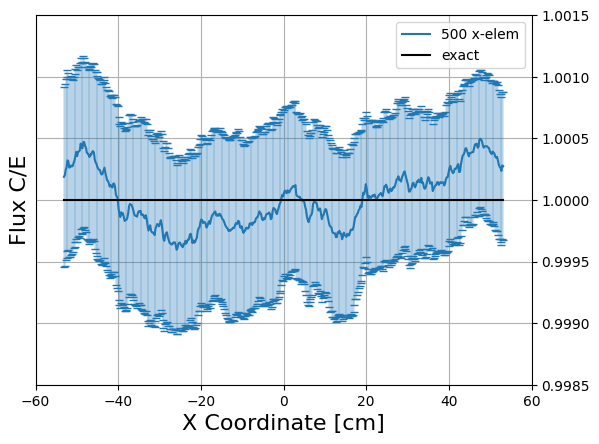
\includegraphics[width=\linewidth]{figures/500_flux_CE_error_bars}
        \caption{$N=500$}
        \label{fig:s4}
    \end{subfigure}
    \par\bigskip
    \begin{subfigure}{0.405\textwidth}
        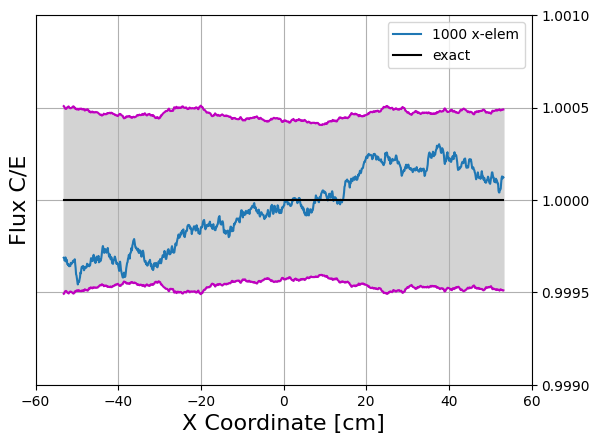
\includegraphics[width=\linewidth]{figures/1000_flux_CE_error_bars}
        \caption{$N=1000$}
        \label{fig:s5}
    \end{subfigure}
    \par\medskip
    \caption{$C/E$ in blue with $2\sigma$ error bars (gray bounded by purple).}
\label{fig:ce_error_bars}
\end{figure}

At this point, the observant reader may be wondering why the fine cases all appear to have about the same errors in $C/E$ despite using smaller and
smaller tally regions. In Monte Carlo, decreasing the volume of a tally region generally causes there to be greater relative error with the same number
of histories. This seemingly counter-intuitive result is rooted in the benchmark itself. The slab domain length is $L=106.47$ cm; however, the \gls{mfp}
ranges between $239$ cm for $T=308$ K and $278$ cm for $T=358$ K. This means the average particle track will transport a particle from the source birth
position to a vacuum boundary condition. Pair that with a spatially uniform birth distribution, and this essentially causes each cell to gain an equal
number of contributions to its neighbors; since this happens in each case, the relative error in each case stays about constant.

The $k$-eigenvalue for each simulation is reported in Table \ref{tab:data}. The results show close agreement with the analytical solution, as all
fine cases agree within $4$ pcm. The coarse cases range from $6$ to $67$ pcm difference. The eigenvalues generally agree better as more mesh elements
are used. The only exception being that the $N=100$ case agrees the best (less than 1 pcm difference from the analytical). The quality agreement is due to
\keff\ being a system-wide parameter which is less sensitive to spatial discretization of temperature feedback than the flux distribution itself.

\begin{table}[H]
    \centering
    \caption{Eigenvalue with uncertainty for each mesh size, and the difference from the analytical.}
    \begin{tabular}{@{}ccc@{}}
        \toprule
        Resolution &  \keff & (numerical - analytical) [pcm]\\
        \midrule
        analytical & 0.29557 & - \\
        \midrule
        5    & 0.29624 $\pm$ 0.00003 & \phantom{-}67 $\pm$ 3 \\
        10   & 0.29581 $\pm$ 0.00004 & \phantom{-}24 $\pm$ 4 \\
        25   & 0.29563 $\pm$ 0.00004 & \phantom{-}6  $\pm$ 4 \\
        50   & 0.29553 $\pm$ 0.00004 &           -4  $\pm$ 4 \\
        100  & 0.29557 $\pm$ 0.00003 & \phantom{-}0  $\pm$ 3 \\
        250  & 0.29561 $\pm$ 0.00004 & \phantom{-}4  $\pm$ 4 \\
        500  & 0.29561 $\pm$ 0.00004 & \phantom{-}4  $\pm$ 4 \\
        1000 & 0.29558 $\pm$ 0.00004 & \phantom{-}1  $\pm$ 4 \\
    \bottomrule
    \end{tabular}
    \label{tab:data}
\end{table}

\section{CONCLUSIONS}\label{sec:conclusions}
Overall, the numerical results show agreement with the analytical solutions. The convergence is first order for the temperature and the $C/E$ for the fluxes
contain the analytical solution for nearly every point within $2\sigma$ across all fine cases. The eigenvalue also agrees very well for all cases.

While experimental benchmarking is critical for nuclear \gls{ms}, agreement with analytical benchmarks also serves an important purpose by increasing confidence
in multiphysics coupling. Though typical industry-grade simulations would not run $S_{2}$ transport, this modification allows Cardinal to be compared against a
theoretical problem. A companion paper in this conference with Cardinal \cite{aya2023} couples OpenMC Monte Carlo transport to NekRS heat conduction. In future
work, we will extend our computational model to include NekRS providing the heat conduction solution.

\section*{ACKNOWLEDGEMENTS}
The authors would like to thank the OpenMC and MOOSE development teams for their guidance in model setup and assistance with software. We also want to thank
Dr. Griesheimer and Dr. Kooreman for their modeling advice and knowledge about the analytical benchmark.

The first author was supported in part by the US Nuclear Regulatory Commission's Graduate Fellowship Program administered by the University of Wisconsin-Madison.
Regarding the second and third authors, the submitted manuscript has been created by UChicago Argonne, LLC, Operator of Argonne National Laboratory (“Argonne”).
Argonne, a U.S. \gls{doe} Office of Science laboratory, is operated under Contract No. DE-AC02-06CH11357. The U.S. Government retains for itself, and others
acting on its behalf, a paid-up nonexclusive, irrevocable worldwide license in said article to reproduce, prepare derivative works, distribute copies to the
public, and perform publicly and display publicly, by or on behalf of the Government. The \gls{doe} will provide public access to these results of federally
sponsored research in accordance with the DOE Public Access Plan. This material is based upon work supported by Laboratory Directed Research and Development
(LDRD) funding from Argonne National Laboratory, provided by the Director, Office of Science, of the U.S. \gls{doe} under Contract No. DE-AC02-06CH11357.

\setlength{\baselineskip}{12pt}
\bibliographystyle{mc2023}
\bibliography{mc2023}
\setlength{\baselineskip}{12pt}

\end{document}
